%%%%%%%%%%%%%%%%%%%%%%%%%%%%%%%%%%%%%%%%%%%%%%%%%%%%%%%%%%
%%                                                      %%
%%             ARTICULO CON FORMATO IEEE                %%
%%                                                      %%
%%%%%%%%%%%%%%%%%%%%%%%%%%%%%%%%%%%%%%%%%%%%%%%%%%%%%%%%%%
%%                                                      %%
%%   Si hace falta otro formato, generar otro archivo   %%
%%  main_format.tex y compilar ese archivo.             %%
%%                                                      %%
%%%%%%%%%%%%%%%%%%%%%%%%%%%%%%%%%%%%%%%%%%%%%%%%%%%%%%%%%%
\documentclass[hidelinks, conference]{IEEEtran}
\IEEEoverridecommandlockouts
% The preceding line is only needed to identify funding in the first footnote. If that is unneeded, please comment it out.
%\usepackage{cite}

%%%%%%% DEPENDENCIAS %%%%%%%
\usepackage{svg}
\usepackage{amsmath,amssymb,amsfonts}
\usepackage{algorithmic}
\usepackage{graphicx}
\usepackage{textcomp}
\usepackage{xcolor}
\usepackage{orcidlink}
\usepackage{hyperref} %<--- Load after everything else


%%%%%% BIBLATEX %%%%%%
\usepackage[style=ieee]{biblatex} %Imports biblatex package
\addbibresource{referencias.bib} %Import the bibliography file
\def\BibTeX{{\rm B\kern-.05em{\sc i\kern-.025em b}\kern-.08em
    T\kern-.1667em\lower.7ex\hbox{E}\kern-.125emX}}

%%%%%% FORMATO - LISTADO DE CADENAS DE BÚSQUEDA %%%%%%
\usepackage{listings}
\lstdefinestyle{cadena_busqueda_style}{
    basicstyle=\ttfamily\footnotesize,
    breakatwhitespace=false,         
    breaklines=true,                 
    captionpos=b,                    
    keepspaces=true,                 
    numbersep=5pt,                  
    showspaces=false,                
    showstringspaces=false,
    showtabs=false,                  
    tabsize=2
}
\lstset{style=cadena_busqueda_style}

%%%%%%% Ajustes de separación de sílabas %%%%%%%
\pretolerance=2000
\tolerance=3000
%\hyphenation{his-to-lo-gy}
%\hyphenation{his-to-pa-tho-lo-gy}
%\hyphenation{re-po-si-to-ry}
%\hyphenation{re-po-si-to-ries}

%%%%%% PARA EL FORMATO DE LAS TABLAS %%%%%%
\usepackage{longtable}
\usepackage{tabularx}
    \newcolumntype{L}{>{\raggedright\arraybackslash}m}
    %\newcolumntype{M}[1]{>{\centering\arraybackslash}m{#1}}
    \newcolumntype{M}{>{\centering\arraybackslash}m}
    \newcolumntype{C}{>{\centering\arraybackslash}p}

\usepackage{array,booktabs,caption,siunitx}

%%%%%% COMANDO PARA COMENTAR BLOQUES DE CÒDIGO %%%%%%
\newcommand{\commentcode}[1]{}


%%%%%%%%%%%%%%%%%%%%%%%%%%%%%%%%%%%%%%%%%%%%%%%%%%%%%%
%   TÍTULO
%%%%%%%%%%%%%%%%%%%%%%%%%%%%%%%%%%%%%%%%%%%%%%%%%%%%%%
\title{Requirements and Challenges to use Explainable Artificial Intelligence in Histopathology: A Rapid Review}

%%%%%%%%%%%%%%%%%%%%%%%%%%%%%%%%%%%%%%%%%%%%%%%%%%%%%%
%   AUTORES
%%%%%%%%%%%%%%%%%%%%%%%%%%%%%%%%%%%%%%%%%%%%%%%%%%%%%%

% $^{\textsuperscript{\orcidicon{0000-0001-7749-5214}}}$

\author{
    \IEEEauthorblockN{
        Juan Cristian Miguel \orcidlink{0000-0001-7749-5214}\IEEEauthorrefmark{1},
        Christian Grévisse \orcidlink{0000-0002-9585-1160}\IEEEauthorrefmark{4},
        Antonia Sardella \IEEEauthorrefmark{4},
        Maria F Pollo-Cattaneo \orcidlink{0000-0003-4197-3880}\IEEEauthorrefmark{1}
    }
    \IEEEauthorblockA{\IEEEauthorrefmark{1}\textit{Facultad Regional Buenos Aires}\\\textit{Universidad Tecnológica Nacional}\\Buenos Aires, Argentina\\\{jmiguel, fpollo\}@frba.utn.edu.ar}
    \IEEEauthorblockA{\IEEEauthorrefmark{4}\textit{Faculty of Science, Technology and Medicine}\\\textit{University of Luxembourg}\\Esch-sur-Alzette, Luxembourg\\christian.grevisse@uni.lu, antonia.sardella@ext.uni.lu}
}


\begin{document}
\maketitle
%%%%%%%%%%%%%%%%%%%%%%%%%%%%%%%%%%%%%%%%%%%%%%%%%%%%%%
%   INCLUSIÓN DE CONTENIDO
%%%%%%%%%%%%%%%%%%%%%%%%%%%%%%%%%%%%%%%%%%%%%%%%%%%%%%
\begin{abstract}
% Un abstract suele ser un resumen del trabajo que presentarás, pero, más importante aún, tiene que ser el “vendedor” que convence al lector (y antes al revisor!) de lo que sigue. Tu mismo has hecho el ejercicio de una revisión, y sabes de lo importante que puede ser el abstract para convencerte de incluir un artículo en algo. De esa misma experiencia puedes deducir cómo escribir un abstract que vende tu artículo. Intenta algo y luego revisamos.

The number of professional pathologists is not high in contrast with the total population, and, worldwide, the cases of cancer have a tendency to rise each year. In the face of this, the implementation of Artificial Intelligence (AI) and, more specifically, Explainable Artificial Intelligence (xAI) techniques could contribute to prevent a work overload on pathologists. Despite recent advances in this subject, AI/xAI systems are still not fully integrated in the histopathology workflow. This could be due to the fact that the implementation of AI/xAI models in histopathology is subject to technical, social and legal requirements, among others. It is necessary to determine these requirements in order to solve this issue. With the intention of providing a wider picture, this article will present a rapid literature review bringing together all current requirements and obstacles that the implementation of AI/xAI faces in histopathology.
\end{abstract}


\begin{IEEEkeywords}
xAI, Digital Pathology, Computational Pathology, Histology, Histopathology
\end{IEEEkeywords}
%%%%%%%%%%%%%%%%%%%%%%%%%%%%%%%%%%%%%%%%%%%%%%%%%%%%%%
%   INTRODUCCIÓN
%%%%%%%%%%%%%%%%%%%%%%%%%%%%%%%%%%%%%%%%%%%%%%%%%%%%%%
\section{Introduction} \label{section:en/introduccion}

Artificial Intelligence (AI) is a type of technology that has been developed substantially in recent years. With the advent of Deep Learning (DL), there are more studies and newly discovered applications of these models in different areas. Most of AI algorithms are based on black box models, which render the traceability unclear on how the result was obtained. In general terms, it can be said that, the more complex the AI model, the harder it is to interpret its results. 
%This is evident when the algorithms are compared to decision trees and neural networks. 
A clear example of this is neural networks, widely used today.
On the other hand, opposed to black box models, there exist white box models, whose intention is to guarantee a clear and direct understanding of the process \cite{Ye2021}.

It has been proved that the implementation of black box models of AI does yield good results in diverse fields of application \cite{Verma2023}. However, in histopathology, applying them as part of the Computer-Aided Diagnosis (CAD) is still a difficult task, due to specific requirements of this field that need to be met, among which the lack of transparency of the process becomes its main obstacle \cite{Abdelsamea2022}. To counter this, numerous techniques known as Explainable Artificial Intelligence (xAI) have been developed, including post-hoc and ante-hoc models. It consists of a collection of processes and methods which allow users to comprehend how an AI algorithm reached a certain result \cite{Giuste2023}. Through these xAI techniques, it is possible to obtain more qualitative evidence of the predictions made by the AI algorithm.

Today, the number of professional pathologists is not high in contrast with the total population, and, worldwide, the cases of cancer have a tendency to rise each year \cite{Zehra2023}. In the face of this, the implementation of AI could contribute to prevent a work overload on pathologists \cite{Liu2021}. Nevertheless, despite the multiple xAI techniques, these are not enough to implement AI models in histopathology, given the lack of a clear consensus in the area. Some researchers support that the method through which an AI analyzes the behavior of an algorithm does not consist of explications or predictions, but rather determining the presence of biases in obtaining them \cite{Ahmad2018}. There exists, furthermore, a debate surrounding the use of post-hoc xAI models (black box) and ante-hoc xAI models: the explanations obtained by a black box do not align with the real process an AI model uses to predict its results, an aspect that provokes certain skepticism when it comes to incorporating these technologies into high-stakes scenarios \cite{Ahmad2018}. AI/xAI systems must also be consistent with its results: it must be able to reproduce or recognize each result in the same manner.

Some authors also declare that doctors and healthcare professionals seek to bond with the systems as if they were colleagues, consulting with them their medical point of view, their experiences and weaknesses, and how to better complement their abilities \cite{Cai2019}. In addition, the implementation of AI/xAI models in histology is subject to technical, social and legal requirements.

With the intention of providing a wider picture, this article will present a rapid literature review bringing together all modern requirements and obstacles that the implementation of AI/xAI faces in histopathology.

This article is structured as follows: Section \ref{section:en/protocolo} describes the research protocol used for the rapid review. In Section \ref{section:en/resultados}, results obtained are analyzed and an answer is provided to the question that drives this review. Finally, in Section \ref{section:en/conclusiones}, conclusions are presented. 

%\section{Background Concepts} \label{section:en/background}
DESCARTADO
%%%%%%%%%%%%%%%%%%%%% SECTION %%%%%%%%%%%%%%%%%%%%%%%
\section{Rapid Review research protocol} \label{section:en/protocolo}

This section describes the research protocol used for this rapid review. Rapid Reviews (RR) are practice-oriented secondary studies, and their main goal is to provide evidence to support decision-making towards the solution, or at least attenuation, of issues practitioners face in practice \cite{Cartaxo2020}.

For this Rapid Review, the PRISMA \cite{Tricco2019} methodology was used for reference. The research question for the case study of this work, the repositories used for the search, the search process and search string, the inclusion and exclusion criteria and the selection process are specified as follows.


%%%%%%%%%%%%%%%%%%%% SECTION %%%%%%%%%%%%%%%%%%%%%%%
\subsection{Research Question}

The Research Question to be answered is the following: \emph{What are the main factors that limit the implementation of AI/xAI in histopathology?} Considering all of the impediments reported so far will permit to gather all of the known and necessary requirements to implement AI/xAI in histopathology. 




%%%%%%%%%%%%%%%%%%%% SECTION %%%%%%%%%%%%%%%%%%%%%%%
\subsection{Search Process and Search string} \label{section:en/search_process}

An automatic search in the ACM, IEEE Xplore, PubMed and Springer digital libraries and platforms was conducted.

For the construction of the search string, the main terms “explainable artificial intelligence”, “histopathology”, “histology” and “anatomic pathology” were considered, including their alternative terms. The resulting search string is presented in Figure \ref{figura:en/cadena_generica}.

\begin{figure}[htbp]
\centering
\begin{tabular}{c}
\begin{lstlisting}
#FULL TEXT
  "xai" OR
  "explainable artificial intelligence" OR
  "explainable ai" OR
  "interpretable ai" OR
  "interpretable artificial intelligence" OR
  "white box" OR
  "human ai"
#AND
#FULL TEXT
  "histopathology" OR
  "histopathological" OR
  "histology" OR
  "histological" OR
  "anatomic pathology" OR
  "anatomical pathology"
\end{lstlisting}
\end{tabular}
\caption{Search string defined for the research}
\label{figura:en/cadena_generica}
\end{figure}



%%%%%%%%%%%%%%%%%%%% SECTION %%%%%%%%%%%%%%%%%%%%%%%
\subsection{Inclusion and exclusion criteria} \label{section:en/inc_exc_criteria}


Since 2015, it has been observed an increment of xAI techniques applied to AI clinical decision support systems \cite{Giuste2023}. Based on these dates, the inclusion criteria was defined as follows: articles published in English between January 2015 and June 2023, in journals or conferences that underwent peer review, and whose main focus is the implementation of AI/xAI in histology or histopathology. Duplicate articles, surveys, systematic reviews and other rapid reviews were excluded for this study.



%%%%%%%%%%%%%%%%%%%% SECTION %%%%%%%%%%%%%%%%%%%%%%%
\subsection{Selection and Data Extraction process} \label{section:en/selection_data_process}

The study selection process consisted of ten steps, which were executed sequentially. Details about the process are described in Figure \ref{figura:en/data_extraction}. This process allowed the selection of the primary studies that were analyzed to answer the research question. The PRISMA checklist used in this study is presented in Appendix \ref{appendix:en/prisma_checklist}.

The search string was applied in the digital libraries with some necessary adjustments depending on the particularities of each one.

\begin{figure}[htbp]
    \centering
%    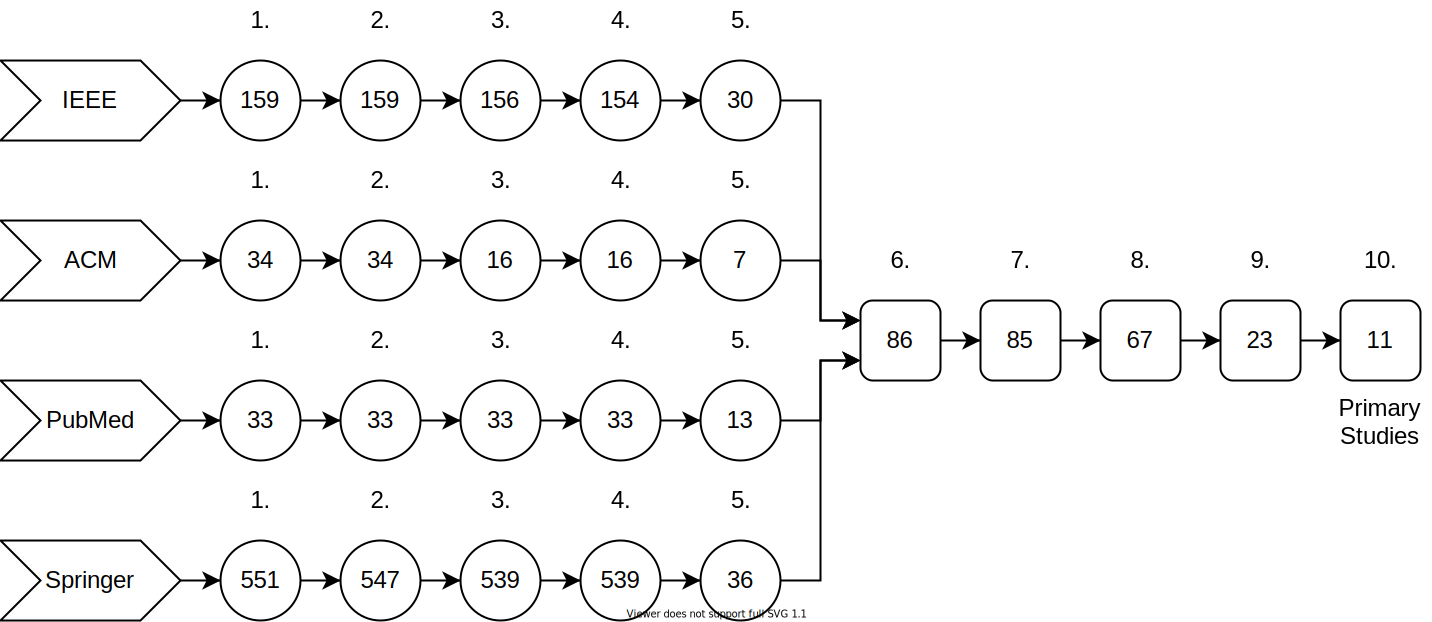
\includegraphics[width=\textwidth]{Imagenes/RR_Steps.svg}
    \includesvg[inkscapelatex=false, width=0.5\textwidth]{Imagenes/RR_Steps_v2.svg}
    \caption{Articles search and selection process details.}
    \label{figura:en/data_extraction}
\end{figure}

For this rapid review, one researcher read the titles, abstracts, and full texts to assess their inclusion. Of a total of 777 articles found, 11 primary studies were analyzed. The list of the selected studies is presented in Appendix \ref{appendix:en/estudios_primarios}.
  %% Version 1
%%%%%%%%%%%%%%%%%%%% SECTION %%%%%%%%%%%%%%%%%%%%%%%
\section{Rapid Review research protocol} \label{section:en/protocolo}

This section describes the research protocol used for this rapid review. Rapid Reviews (RR) are practice-oriented secondary studies, and their main goal is to provide evidence to support decision-making towards the solution, or at least attenuation, of issues practitioners face in practice \cite{Cartaxo2020}.

For this Rapid Review, the PRISMA \cite{Tricco2019} methodology was used for reference. The research question for the case study of this work, the repositories used for the search, the search process and search string, the inclusion and exclusion criteria and the selection process are specified as follows.


%%%%%%%%%%%%%%%%%%%% SECTION %%%%%%%%%%%%%%%%%%%%%%%
\subsection{Research Question}

The Research Question to be answered is the following: \emph{What are the main factors that limit the implementation of AI/xAI in histopathology?} Considering all of the impediments reported so far will permit to gather all of the known and necessary requirements to implement AI/xAI in histopathology. 




%%%%%%%%%%%%%%%%%%%% SECTION %%%%%%%%%%%%%%%%%%%%%%%
\subsection{Search Process and Search string} \label{section:en/search_process}

An automatic search in the ACM, IEEE Xplore, PubMed and Springer digital libraries and platforms was conducted.

For the construction of the search string, the main terms “explainable artificial intelligence”, “histopathology”, “histology” and “anatomic pathology” were considered, including their alternative terms. The resulting search string is presented in Figure \ref{figura:en/cadena_generica}.

\begin{figure}[htbp]
\centering
\begin{tabular}{c}
\begin{lstlisting}
#FULL TEXT
  "xai" OR
  "explainable artificial intelligence" OR
  "explainable ai" OR
  "interpretable ai" OR
  "interpretable artificial intelligence" OR
  "white box" OR
  "human ai"
#AND
#FULL TEXT
  "histopathology" OR
  "histopathological" OR
  "histology" OR
  "histological" OR
  "anatomic pathology" OR
  "anatomical pathology"
\end{lstlisting}
\end{tabular}
\caption{Search string defined for the research}
\label{figura:en/cadena_generica}
\end{figure}



%%%%%%%%%%%%%%%%%%%% SECTION %%%%%%%%%%%%%%%%%%%%%%%
\subsection{Inclusion and exclusion criteria} \label{section:en/inc_exc_criteria}


Since 2015, it has been observed an increment of xAI techniques applied to AI clinical decision support systems \cite{Giuste2023}. Based on these dates, the inclusion criteria was defined as follows: articles published in English between January 2015 and June 2023, in journals or conferences that underwent peer review, and whose main focus is the implementation of AI/xAI in histology or histopathology. Duplicate articles, surveys, systematic reviews and other rapid reviews were excluded for this study.



%%%%%%%%%%%%%%%%%%%% SECTION %%%%%%%%%%%%%%%%%%%%%%%
\subsection{Selection and Data Extraction process} \label{section:en/selection_data_process}

The study selection process consisted of ten steps, which were executed sequentially. Details about the process are described in Figure \ref{figura:en/data_extraction}. This process allowed the selection of the primary studies that were analyzed to answer the research question. The PRISMA checklist used in this study is presented in Appendix \ref{appendix:en/prisma_checklist}.

The search string was applied in the digital libraries with some necessary adjustments depending on the particularities of each one.

\begin{figure}[htbp]
    \centering
%    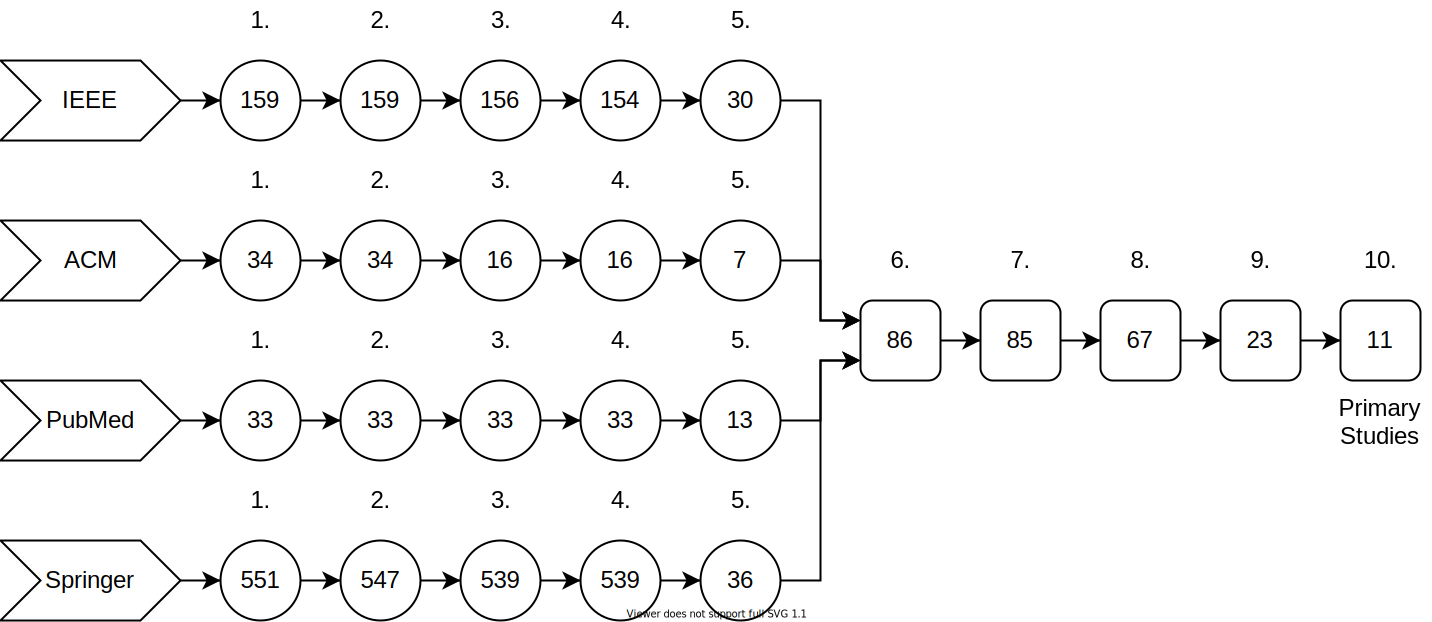
\includegraphics[width=\textwidth]{Imagenes/RR_Steps.svg}
    \includesvg[inkscapelatex=false, width=0.5\textwidth]{Imagenes/RR_Steps_v2.svg}
    \caption{Articles search and selection process details.}
    \label{figura:en/data_extraction}
\end{figure}

For this rapid review, one researcher read the titles, abstracts, and full texts to assess their inclusion. Of a total of 777 articles found, 11 primary studies were analyzed. The list of the selected studies is presented in Appendix \ref{appendix:en/estudios_primarios}.
   %% Version 2
%%%%%%%%%%%%%%%%%%%% SECTION %%%%%%%%%%%%%%%%%%%%%%%
\section{Review Results} \label{section:en/resultados}

This section aims to answer the research question based on the analysis performed on the primary studies. We identified five classes of challenges that the implementation of AI/xAI must face in histopathology: technical difficulties, process transparency, coupling workflow, implementation costs and regulation aspects. 






%%%%%%%%%%%%%%%%%%%% SECTION %%%%%%%%%%%%%%%%%%%%%%%
\subsection{Technical difficulties}
% Sesgos, disparidad entre los datasets, diferencias de formatos, diferencia entre equipos WSI, etc...

In supervised AI systems, it is crucial to rely on datasets whose samples are classified by an expert with the intention of obtaining consistent predictions. However, many authors declare there are operative difficulties when classifying.

Ayorinde et al. \cite{Ayorinde2022} analyze that a reliable categorization can be problematic for some elements of slide assessment, especially in determination of arteriosclerosis. Arteriosclerosis is recognized by the narrowing of the blood vessel lumen, although this is not always the case: an apparently narrow lumen may arise not only from disease but also from oblique sectioning. Thus, when processing blood vessel slides, the similarity between them becomes a critical issue for AI implementation due to the possibility of arriving at an erroneous diagnosis. 

Tran et al. \cite{Tran2021} remark that this is also limiting in oncology, and that it is currently unclear how DL systems would deal with this inter- and intra-laboratory variability. They also add that, in many DL systems, the predictions are simply the best guess with the highest probability. In critical circumstances, overconfident predictions, e.g. predicting cancer primary site with only 40\% certainty, can result in inaccurate diagnosis or cancer management decisions.

Along these lines, Mohammadi et al. \cite{Mohammadi2022}, mention that a fully supervised learning for whole slide image–based diagnostic tasks in histopathology is problematic due to the requirement for costly and time-consuming manual annotation by experts, and propose the use of weakly supervised learning methods in order to reduce costs at scale. When it comes to processing, Mohammadi et al. comment that training AI models on gigapixel size whole-slide images is highly expensive and that they usually resort to patching approaches.

Dos-Santos et al. \cite{dosSantos2022} state that the lack of diversity in datasets is another difficulty that AI systems face. Moreover, the datasets must be in some way linked to clinical patient data to allow the validation of external algorithms, in addition to morphological validations performed by pathologists.

An important aspect to consider is the data privacy of the patients. On this, Rösler et al. \cite{Roesler2023} say that data in medicine must be securely stored, transferred, and protected from unauthorized access.

On the other hand, Holzinger et al. \cite{Holzinger2019}, reflect on the fact that oftentimes the datasets are not “big” enough. They observe that there is an inherent tension between ML performance (predictive accuracy) and explainability. Often the best-performing AI models are the least transparent, and the ones providing a clear explanation are less accurate.

%%%%%%%%%%%%%%%%%%%% SECTION %%%%%%%%%%%%%%%%%%%%%%%
\subsection{Process transparency}
% Transparencia, interpretabilidad, causability

Explainability is considered one of the prerequisites for AI in medicine. In this sense, xAI is seen as a step towards the realization of the FATE principles in AI \cite{ShabanNejad2021}.

Holzinger et al. \cite{Holzinger2019} propose that it is necessary to understand the causality of representations. This is why they differentiate the words “explainability” and “causality”. Explainability highlights decision-relevant parts of the used representations of the algorithms and active parts in the algorithmic model and it does not refer to an explicit human model. Causability is defined as the extent to which an explanation of a statement to a human expert achieves a specified level of causal understanding in a specified context of use. Establishing causability as a solid scientific field becomes imperative in this sense.

%%%%%%%%%%%%%%%%%%%% SECTION %%%%%%%%%%%%%%%%%%%%%%%
\subsection{Coupling workflow}
% AI no como reemplazo. AI no reemplaza la histologìa manual

Ayorinde et al. \cite{Ayorinde2022} postulate that it is not necessary to achieve a perfect AI system for it to be used in the hospitals. In fact, it is more probable that the most useful tools are a combination between AI models and a set of work rules that favor the effective human supervision.

According to Tosun et al. \cite{Tosun2020} the main function of xAI in pathology is to promote safety, reliability, and accountability in addressing issues with bias, transparency, safety, and causality. The authors find, however, that there is not yet a consensus on how pathologists should supervise or work with computational pathology systems. As patient safety in pathology is the result of a complex interaction between pathologists, other physicians, laboratory personnel and computational pathology applications, they conclude that xAI must help the pathologist be more precise and efficient in their work.

Jaharri et al. \cite{Jarrahi2022} claim that the AI/xAI systems employed in medicine present interoperability challenges, given that these systems often show an amount of information or in formats that appear indecipherable to physicians. These authors offer that an expert-in-the-loop AI work system could clarify a mutual workflow between humans and machines.

As for Verma et al. \cite{Verma2023}, they suggest that AI can be included in collective decision-making processes in oncology either as a tool or as a member, each of these alternatives generating different sets of ethical, societal and technological issues. In an interview they conducted for their article \cite{Verma2023} with seven physicians working at the Lausanne University Hospital (CHUV), in relation to AI systems autonomy, they detected a consensus on how trust cannot be put in something that is not trustful or bypasses the doctors. One of the experts that took part in this interview added that an AI model cannot be trusted if it is not able to choose which treatment modality works best for a particular patient.

%%%%%%%%%%%%%%%%%%%% SECTION %%%%%%%%%%%%%%%%%%%%%%%
\subsection{Implementation costs}
% Acerca de LMIC

Zehra et al. \cite{Zehra2023} analyze the implementation of AI in low- and middle-income countries (LMICs). They remark that, while AI systems there face similar technical challenges and issues to those of more developed countries, there are further difficulties in LMICs. The authors perceive that when labs struggle due to financial constraints to hire trained histopathologists, and when there is scarcity of trained laboratory technologists even for conventional histopathology, it would be extremely difficult to obtain funds and manpower for implementing AI and digital pathology. In the face of this, they propose a series of low-cost alternatives to venture into AI systems. For instance, low resource organizations can access available open-source whole-slide image archives provided by the Cancer Genome Atlas \cite{CancerGenomeAtlasWebsite}, the Cancer Imaging Archive \cite{CancerImagingArchiveWebsite} and the Digital Pathology Association’s Whole-Slide Imaging Repository \cite{DAPAWebsite}, among others. Another alternative would be when facing internet glitches and the downloading of these images provided by these repositories. As they are large in size, many of the professionals in LMICs may find it difficult to obtain the data for the AI training. To solve this issue, Pathologists can photograph a region of interest for a particular pathology by using the data of their own patients. After taking the photograph, these images can be classified and uploaded in AI systems either open-source or commercially available, although the latter are usually expensive.

%%%%%%%%%%%%%%%%%%%% SECTION %%%%%%%%%%%%%%%%%%%%%%%
\subsection{Regulation aspects}
% En caso de confiar en un algoritmo de AI que brinda un diagnòstico equivocado, ¿quién es responsable bajo la ley?
% Privacidad de datos. Datasets públicos vs historia clínica de los pacientes (privada por default)

In relation to regulations, Tosun et al. \cite{Tosun2020} reveal that a proposed regulation before the European Union would prohibit “automatic processing” unless people are safeguarded. They foresee that future laws may further restrict AI use in professional practices, which represents a huge challenge to industry.

Dos-Santos et al. \cite{dosSantos2022} affirm that AI algorithms must work under regulatory standards for testing and usage in medical facilities. According to Tosun et al. \cite{Tosun2020}, this is already a known necessity in radiology.

Thus, due to data privacy, Rösler et al. \cite{Roesler2023} observe that professionals must work under an ethical approval and informed consent of the patient prior to the use and evaluation of patient-related data. In addition to this, if possible, anonymized raw data have to be included from the start of the training process.

\section{Conclusions and Future work} \label{section:en/conclusiones}

Though the implementation of AI/xAI seems promising, this article brings to light the challenges that must be solved so that an effective implementation of these technologies may take place in histopathology. These difficulties are not limited to technical ones only, but they also cover other equally important perspectives.

The coupling workflow is the main factor that must be considered when designing an AI system. It is necessary to establish a list of requirements with specialists and pathologists with the purpose of understanding their needs and finding the best way they can benefit themselves from these technologies. AI/xAI systems must be conceived as assistants to pathologists, and allow for sufficient transparency so their results can be supervised. 
It is possible that, to achieve an adequate integration with the workflow, it is vital to incorporate the expert-in-the-loop approach. Another possibility is to consider AI/xAI algorithms like components of a more complex system that implements pieces of traditional programming and results expressed in natural language. With the recent advent of Large Language Models (LLM), the aforementioned bonding between pathologists and xAI systems could be enhanced.

AI/xAI systems are highly sensitive to the quality of their data. Adequately classified samples are crucial for the success of the AI training. Due to this task being exhaustive, it may be accelerated by resorting to weakly supervised learning methods. However, to obtain a precise classification in oncology and renal histopathology sometimes is complex. In the face of this difficulty, designing AI systems from an approach centered in causability instead of explainability might contribute significantly to the professionals. 

There is still a necessity for a set of regulations that guarantee a standard in relation to the testing and the use of AI systems in histopathology, in the case that these systems require the utilization of patient-related data for training.

The cost of implementation is also a limiting factor in some organizations. Against this, open-source alternatives might become the starting point for the implementation of AI-based solutions.

As for the next steps of this article, this work will be expanded to create a systematic mapping study of literature. It is expected for this to be the foundations of a future investigation.
\appendices

%%%%%%%%% SECTION %%%%%%%%%
\section{PRISMA Checklist} \label{appendix:en/prisma_checklist}

The PRISMA checklist used for this review is presented in Table \ref{tabla:en/prisma_checklis}

\begin{table*}
%\begin{landscape}
\caption{PRISMA Checklist}
\begin{center}
\begin{tabularx}{\hsize}{M{2.3cm}|M{0.7cm}|M{10cm}|M{3cm}}
\hline
\textbf{Section and Topic} & \textbf{Item} & \textbf{Checklist item} & \textbf{Location where item is reported} \\
\hline
\hline
\multicolumn{4}{l}{\textbf{Title}} \\
\hline
Title & 1 & Identify the report as a systematic review. & Title \\
\hline
\hline
\multicolumn{4}{l}{\textbf{Abstract}} \\
\hline
Abstract & 2 &  See the PRISMA 2020 for Abstracts checklist. & Abstract \\
\hline
\hline
\multicolumn{4}{l}{\textbf{Introduction}} \\
\hline
Rationale & 3 &Describe the rationale for the review in the context of existing knowledge.& Section \ref{section:en/introduccion}\\
\hline
Objectives &4& Provide an explicit statement of the objective(s) or question(s) the review addresses. & Section \ref{section:en/introduccion}\\
\hline
\hline
\multicolumn{4}{l}{\textbf{Methods}} \\
\hline
Eligibility criteria &5&  Specify the inclusion and exclusion criteria for the review and how studies were grouped for the syntheses. & Section \ref{section:en/inc_exc_criteria} \\
\hline
Information sources &6&  Specify all databases, registers, websites, organisations, reference lists and other sources searched or consulted to identify studies. Specify the date when each source was last searched or consulted. & Section \ref{section:en/search_process} \\
\hline
Search strategy & 7&  Present the full search strategies for all databases, registers and websites, including any filters and limits used. & Section \ref{section:en/search_process} \\
\hline
Selection process &8 & Specify the methods used to decide whether a study met the inclusion criteria of the review, including how many reviewers screened each record and each report retrieved, whether they worked independently, and if applicable, details of automation tools used in the process. & Section \ref{section:en/selection_data_process} \\
\hline
Data collection process& 9 & Specify the methods used to collect data from reports, including how many reviewers collected data from each report, whether they worked independently, any processes for obtaining or confirming data from study investigators, and if applicable, details of automation tools used in the process. & Section \ref{section:en/selection_data_process} \\
\hline
Data items &10a & List and define all outcomes for which data were sought. Specify whether all results that were compatible with each outcome domain in each study were sought (e.g. for all measures, time points, analyses), and if not, the methods used to decide which results to collect. & Section \ref{section:en/selection_data_process} \\
\cline{2-4} 
 &10b & List and define all other variables for which data were sought (e.g. participant and intervention characteristics, funding sources). Describe any assumptions made about any missing or unclear information. & Section \ref{section:en/selection_data_process} \\
\hline
Study risk of bias assessment & 11 & Specify the methods used to assess risk of bias in the included studies, including details of the tool(s) used, how many reviewers assessed each study and whether they worked independently, and if applicable, details of automation tools used in the process. & Not included \\
\hline
Effect measures& 12 & Specify for each outcome the effect measure(s) (e.g. risk ratio, mean difference) used in the synthesis or presentation of results. & Not applicable \\
\hline
Synthesis methods &13a & Describe the processes used to decide which studies were eligible for each synthesis (e.g. tabulating the study intervention characteristics and comparing against the planned groups for each synthesis (item 5)). &  Section \ref{section:en/selection_data_process} \\
\cline{2-4} 
 &13b & Describe any methods required to prepare the data for presentation or synthesis, such as handling of missing summary statistics, or data conversions. &  Section \ref{section:en/selection_data_process} \\
\cline{2-4} 
 & 13c & Describe any methods used to tabulate or visually display results of individual studies and syntheses. &  Section \ref{section:en/selection_data_process} and Appendix \ref{appendix:en/estudios_primarios} \\
\cline{2-4} 
 & 13d & Describe any methods used to synthesize results and provide a rationale for the choice(s). If meta-analysis was performed, describe the model(s), method(s) to identify the presence and extent of statistical heterogeneity, and software package(s) used. & Section \ref{section:en/selection_data_process} \\
\cline{2-4} 
 & 13e & Describe any methods used to explore possible causes of heterogeneity among study results (e.g. subgroup analysis, meta-regression). & Section \ref{section:en/search_process} and Section \ref{section:en/selection_data_process} \\
\cline{2-4} 
 & 13f & Describe any sensitivity analyses conducted to assess robustness of the synthesized results. & Not applicable \\
\hline
Reporting bias assessment & 14 & Describe any methods used to assess risk of bias due to missing results in a synthesis (arising from reporting biases). & Not applicable \\
\hline
Certainty assessment & 15 & Describe any methods used to assess certainty (or confidence) in the body of evidence for an outcome. & Not included \\
\hline
\end{tabularx}
\label{tabla:en/prisma_checklis}
\end{center}
\end{table*}


%% SEGUNDA PARTE DE LA TABLA
%% TODO: No pude conseguir que sean la misma tabla
\begin{table*}
%\begin{landscape}
%\caption{PRISMA Checklist}
\begin{center}
\begin{tabularx}{\hsize}{M{2.3cm}|M{0.7cm}|M{10cm}|M{3cm}}
\hline
\textbf{Section and Topic} & \textbf{Item} & \textbf{Checklist item} & \textbf{Location where item is reported} \\
\hline
\hline
\multicolumn{4}{l}{\textbf{Results}} \\
\hline
Study selection & 16a & Describe the results of the search and selection process, from the number of records identified in the search to the number of studies included in the review, ideally using a flow diagram. & Section \ref{section:en/resultados} and Figure \ref{figura:en/data_extraction} \\
\cline{2-4} 
 & 16b & Cite studies that might appear to meet the inclusion criteria, but which were excluded, and explain why they were excluded. & Figure \ref{figura:en/data_extraction} \\
\hline
Study characteristics & 17 & Cite each included study and present its characteristics. & Section \ref{section:en/resultados} \\
\hline
Risk of bias in studies & 18 & Present assessments of risk of bias for each included study. & Not included \\
\hline
Results of individual studies & 19 & For all outcomes, present, for each study: (a) summary statistics for each group (where appropriate) and (b) an effect estimate and its precision (e.g. confidence/credible interval), ideally using structured tables or plots. & Not applicable \\
\hline
Results of syntheses & 20a &  For each synthesis, briefly summarise the characteristics and risk of bias among contributing studies. & Not included \\
\cline{2-4} 
 & 20b & Present results of all statistical syntheses conducted. If meta-analysis was done, present for each the summary estimate and its precision (e.g. confidence/credible interval) and measures of statistical heterogeneity. If comparing groups, describe the direction of the effect. & Not applicable \\
\cline{2-4} 
 & 20c & Present results of all investigations of possible causes of heterogeneity among study results. & Not applicable \\
\cline{2-4} 
 & 20d & Present results of all sensitivity analyses conducted to assess the robustness of the synthesized results. & Not included \\
\hline
Reporting biases & 21 & Present assessments of risk of bias due to missing results (arising from reporting biases) for each synthesis assessed. & Not included \\
\hline
Certainty of evidence & 22 & Present assessments of certainty (or confidence) in the body of evidence for each outcome assessed & Section \ref{section:en/resultados} \\
\hline
\hline
\multicolumn{4}{l}{\textbf{Discussion}} \\
\hline
Discussion & 23a & Provide a general interpretation of the results in the context of other evidence. & Section \ref{section:en/conclusiones} \\
\cline{2-4} 
 & 23b & Discuss any limitations of the evidence included in the review. & Section \ref{section:en/conclusiones} \\
\cline{2-4} 
 & 23c & Discuss any limitations of the review processes used. & Not included \\
\cline{2-4} 
 & 23d & Discuss implications of the results for practice, policy, and future research. & Section \ref{section:en/conclusiones} \\
\hline
\hline
\multicolumn{4}{l}{\textbf{Other information}} \\
\hline
Registration and protocol & 24a & Provide registration information for the review, including register name and registration number, or state that the review was not registered. & Review not registered \\
\cline{2-4} 
 & 24b & Indicate where the review protocol can be accessed, or state that a protocol was not prepared. & Not applicable \\
\cline{2-4} 
 & 24c & Describe and explain any amendments to information provided at registration or in the protocol. & Not applicable \\
\hline
Support & 25 & Describe sources of financial or non-financial support for the review, and the role of the funders or sponsors in the review. & Not applicable \\
\hline
Competing interests & 26 & Declare any competing interests of review authors. & Not declared \\
\hline
Availability of data, code and other materials & 27 & Report which of the following are publicly available and where they can be found: template data collection forms; data extracted from included studies; data used for all analyses; analytic code; any other materials used in the review. & Appendix \ref{appendix:en/estudios_primarios} and References \\
\hline
\end{tabularx}
%\label{tabla:en/prisma_checklis}
\end{center}
\end{table*}
%\end{landscape}




%%%%%%%%% SECTION %%%%%%%%%
\section{List of primary studies} \label{appendix:en/estudios_primarios}

The list of the studies analyzed is presented in Table \ref{tabla:en/estudios_primarios}.

\begin{table*}
\setlength\tabcolsep{0pt}
\caption{List of the primary studies analyzed}
\begin{center}
%\resizebox{\columnwidth}{!}{
%\begin{tabular}{|m{2.5em}|m{20em}|}
\begin{tabularx}{17cm}{C{0.5cm} M{2.5cm} M{1cm} M{8cm} M{5cm}}
\hline
\textbf{ID} & \textbf{Authors} & \textbf{Year} & \textbf{Venue} & \textbf{Category} \\
\hline
\hline
\cite{Ayorinde2022} & Ayorinde et al. & 2022 & Journal of the American Society of Nephrology: JASN & Technical difficulties, Coupling workflow \\
\hline
\cite{dosSantos2022} & Dos-Santos et al. & 2022 & Surgical and Experimental Pathology & Technical difficulties, Regulation aspects \\
\hline
\cite{Holzinger2019} & Holzinger et al. & 2019 & Wiley interdisciplinary reviews. Data mining and knowledge discovery & Technical difficulties, Process transparency \\
\hline
\cite{Jarrahi2022} & Jarrahi et al. & 2022 & Journal of pathology informatics & Coupling workflow \\
\hline
\cite{Mohammadi2022} & Mohammadi et al. & 2022 & Experimental biology and medicine (Maywood, N.J.) & Technical difficulties \\
\hline
\cite{Roesler2023} & Rösler et al. & 2023 & Journal of Cancer Research and Clinical Oncology & Technical difficulties, Regulation aspects \\
\hline
\cite{ShabanNejad2021} & Shaban-Nejad et al. & 2021 & IEEE Journal of Biomedical and Health Informatics & Process transparency \\
\hline
\cite{Tosun2020} & Tosun et al. & 2020 & Advances in anatomic pathology & Coupling workflow, Regulation aspects \\
\hline
\cite{Tran2021} & Tran et al. & 2021 & Genome Medicine & Technical difficulties \\
\hline
\cite{Verma2023} & Verma et al. & 2023 & Proceedings of the 2023 CHI Conference on Human Factors in Computing Systems & Coupling workflow \\
\hline
\cite{Zehra2023} & Zehra et al. & 2023 & Diagnostic Pathology & Implementation costs \\
\hline
\end{tabularx}
\label{tabla:en/estudios_primarios}
\end{center}
\end{table*}





          %% Version 2


%%%%%%%%%%%%%%%%%%%%%%%%%%%%%%%%%%%%%%%%%%%%%%%%%%%%%%
%   REFERENCIAS
%%%%%%%%%%%%%%%%%%%%%%%%%%%%%%%%%%%%%%%%%%%%%%%%%%%%%%
\printbibliography[title={References}]
%\begin{thebibliography}{00}


\end{document}
